\documentclass[12pt,a4paper]{report}

\usepackage{graphicx}

\usepackage[portuguese]{babel}
\usepackage[utf8]{inputenc}

\usepackage{hyperref}
\usepackage{graphicx}
\usepackage{float}
\usepackage{lmodern}

\addto\captionsportuguese{\def\bibname{Referências}}

% Format chapeters
\usepackage[T1]{fontenc}
\usepackage{titlesec, blindtext, color}
\definecolor{gray75}{gray}{0.75}
\newcommand{\hsp}{\hspace{20pt}}
\titleformat{\chapter}[hang]{\Huge\bfseries}{\thechapter\hsp\textcolor{gray75}{|}\hsp}{0pt}{\Huge\bfseries}

\usepackage[parfill]{parskip}
\usepackage{setspace}
\onehalfspacing

\setlength{\abovecaptionskip}{0pt}
%\setlength{\intextsep}{15pt}

\begin{document}
\begin{titlepage}

\newcommand{\HRule}{\rule{\linewidth}{0.5mm}} % Defines a new command for the horizontal lines, change thickness here

\center

% HEADING SECTIONS
\LARGE Universidade dos Açores\\[0.5cm]
\Large Informática - Redes e Multimédia\\[1.5cm]
\large Administração de Sistemas e de Redes\\[0.5cm]

%  TITLE SECTION
\HRule \\[0.4cm]
{ \LARGE \bfseries Serviço de redes para empresa local}\\[0.4cm]
\HRule \\[1.5cm]

%	AUTHOR SECTION
\begin{minipage}{0.4\textwidth}
\begin{flushleft} \large
\emph{Grupo:}\\
\small Helder Correia - 20102556\\
\small Miguel Luís - 20122604\\
\end{flushleft}
\end{minipage}
~
\begin{minipage}{0.4\textwidth}
\begin{flushright} \large
\emph{Professora:}\\
\small Ibéria Medeiros\\
\small iberia@uac.pt
\end{flushright}
\end{minipage}\\[4cm]

%	DATE SECTION
{\Large Projecto Final}\\[0.5cm]
{\large \today}\\[3cm]

\vfill % Fill the rest of the page with whitespace

\end{titlepage}

\tableofcontents

\chapter{Solução}

A solução encontrada para a empresa Imbcc, SA está representada no diagrama da figura~\ref{fig:deployment}.

~
\begin{figure}[H]
\begin{center}
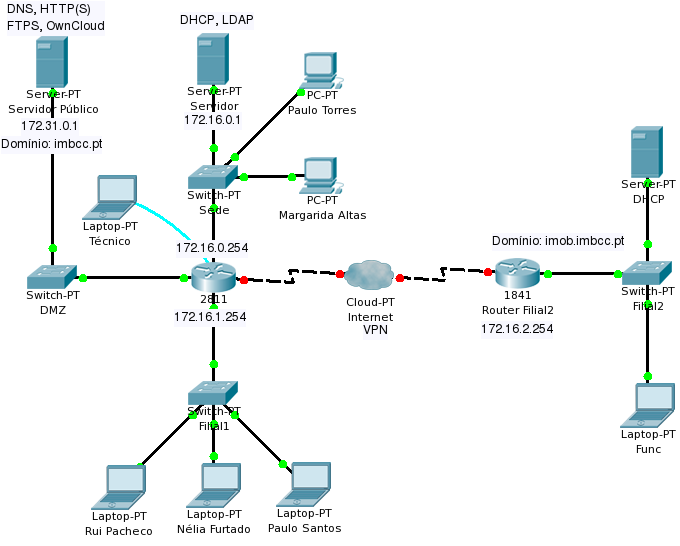
\includegraphics[width=\textwidth]{figs/diagrama-deployment.png}
\end{center}
\caption{Topologia de rede para implementação da solução.}
\label{fig:deployment}
\end{figure}

Para poupar em equipamentos, o router na Sede deve suportar 4 interfaces de rede separadas, nem que seja através de sub-interfaces. O router e dois servidores ficam no armário de equipamentos da Sede. Um servidor é privado, para uso interno enquanto o outro deverá ser acessível externamente, ambos em redes separadas. Uma terceira interface leva um cabo de rede ao piso inferior até a um switch que liga os computadores da Filial 1. Para ligação segura entre a Filial 2 e o resto da empresa no edifício da Sede será usada uma ligação VPN gerida de forma transparente pelo ISP local, que aproveita a linha de acesso à Internet.

Para além do DHCP, o servidor da Sede serve também o serviço de LDAP de forma centralizada e privada (interno). O servidor da rede pública (rede DMZ), contém os serviços de resolução de nomes (DNS), páginas web (HTTP e HTTPS), FTPS para upload dos ficheiros para a web, e é onde fica o ownCloud para que seja possível usar o serviço externamente.

O ownCloud deve ter ligação segura por TLS com o servidor LDAP para a autenticação dos utilizadores da empresa. Todos os computadores devem ter um servidor de SSH com conexões limitadas apenas à equipa técnica para acesso remoto.

\section{DHCP}

O servidor de DHCP na Sede serve 3 redes: a \texttt{sede}, a \texttt{dmz} e a \texttt{filial1}. Um DCHP relay fica activo no router e assim consegue estender o domínio até às outras redes. O servidor principal da DMZ podia receber o seu IP dinamicamente com reserva de atribuição de IP mas o melhor é não depender do outro servidor privado. Assim o servidor da DMZ consegue funcionar de forma independente e também facilita a gestão de serviços como o DNS.

\section{DNS}

O DNS suporta duas vistas. Uma interna e outra externa. A vista interna dá um nome a todos os computadores da empresa. Regra geral, na rede DMZ os servidores têm o nome \verb+serv$+, onde \verb+$+ representa o número do último octeto do IP (e.g. 172.31.0.5 corresponde a \texttt{serv5}). Na Sede e na Filial 2, tendo ambas um servidor privado, têm o nome de \texttt{server}, i.e., \texttt{server.imbcc.pt} e \texttt{server.imob.imbcc.pt} respectivamente.

Para as máquinas que recebem o IP por DHCP, têm o nome \verb+dhcp[rede]$+. O número opcional da rede é para distinguir as máquinas da Sede (com id~0) das máquinas da Filial~1 (com id~1) uma vez que pertencem ao mesmo domínio. Ou seja, sendo que as gamas de IPs são 60-99, o primeiro cliente DHCP da Sede, Filial~1 e Filial~2 são respectivamente \texttt{dhcp060}, \texttt{dhcp160} e \texttt{dhcp60.imob}.

Para fazer o subdomínio da Filial~2 (imob) optou-se não por criar uma zona dedicada mas sim usar o ficheiro de zona principal para facilitar a gestão. Assim cada máquina da Filial~2 tem o sufixo de \texttt{.imob} em frente a cada nome.

Cada nome adicional da mesma máquina é configurado com um registo CNAME na rede interna ou um registo A na rede DMZ. Assim, usando por exemplo a ferramenta \texttt{dig} para questionar o subdomínio \texttt{www} será retornado na resposta o CNAME para serv1 internamente, mas externamente retornará o IP (registo A) do próprio servidor. Na DMZ apenas se usa o CNAME se o serviço for mesmo análogo (como \texttt{dns} ser outro nome para \texttt{ns1}).

Para a tradução reversa de nomes (registos PTR), externamente o servidor da DMZ é visto como \texttt{ns1} principalmente, mas internamente o IP é traduzido para \texttt{serv1}.

A configuração de forwarders facilita a gestão da rede porque as máquinas apenas precisam do servidor DNS da DMZ. A vista \textit{external} tem a opção \textit{recursion} ligada apenas durante a fase de testes para que apenas seja preciso o servidor DNS da DMZ na máquina ligada externamente. Porém em produção essa opção deve ser desligada para não oferecer serviços de DNS gratuitamente ao público geral.

Optou-se por não implementar um servidor de DNS secundário para poupar em equipamento. 

\section{HTTP}

Para os serviços web optou-se por usar o Apache~2, com configuração por \textit{virtual hosts}. Para o site principal da empresa optou-se por preferir o subdomínio \texttt{www} portanto acessos ao endereço \url{http://imbcc.pt} são redireccionados para \url{http://www.imbcc.pt}. É também neste domínio principal que estão configuradas as homepages dos vendedores imobiliários acedendo por exemplo ao endereço \url{http://www.imbcc.pt/~nelia/} para aceder à página da Nélia Furtado.

Com a excepção do serviço ownCloud, há apenas mais um site HTTPS para ligação segura: \url{https://clientes.imbcc.pt}. Os acessos a este endereço com http serão redireccionados automaticamente para a versão segura. Todos os outros acessos a um https que não esteja configurado serão redireccioandos para a sua versão http.

\section{Certificados}

Os certificados são assinados por um CA \textit{self-signed} pertencente à empresa. Esse CA é que assina todos os certificados que são precisos. Esta PKI foi criada usando o TinyCA. As passwords dos certificados (se existirem) é \texttt{imbcc}.

\section{LDAP}

Para a configuração do LDAP foi editado o ficheiro \path{/etc/openldap/slapd.d/cn=config/olcDatabase={2}bdb.ldif} para mudar o \texttt{olcSuffix} e \texttt{olcRootDN}, assim como o \texttt{olcRootPW} com uma password criada com \texttt{sldappasswd -s imbcc}. Também foi editado o ficheiro \path{olcDatabase={1}monitor.ldif} para actualizar o \texttt{base.dn}. O resultado está nos ficheiros de configuração entregues com o projecto.

Depois são adicionados as entradas ao directório usando o \path{ldapadd} e os ficheiros \path{.ldif} também entregues. A ordem é importante. 

\begin{verbatim}
ldapadd -f [ficheiro].ldif -D [valor de olcRootDN] -w [password]

  imbcc.ldif
  users.ldif
  groups.ldif
  users/margarida.ldif
  users/nelia.ldif
  users/paulo.ldif
  users/psantos.ldif
  users/rui.ldif
  groups/webdesign.ldif
  groups/imob.ldif
\end{verbatim}

Para a organização da árvore LDAP usou-se os \emph{organizational units} para representar um tipo de objectos. Temos um para os utilizadores todos e outro para os grupos. Posteriormente pode ser criado mais um para os equipamentos por exemplo. Depois dentro do \texttt{ou=groups} temos os grupos do web designers e dos utilizadores da imobiliária. Cada grupo depois tem como membro os utilizadores adequados do \texttt{ou=users}. Este esquema pode ser visualizado com a figura~\ref{fig:ldaptree}.

\begin{figure}[H]
\begin{center}
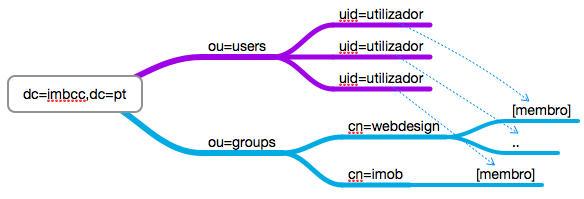
\includegraphics[width=\textwidth]{figs/ldap-tree.png}
\end{center}
\caption{Esquema da árvore LDAP para esta empresa.}
\label{fig:ldaptree}
\end{figure}

O nome mais descritivo dos grupos pode ser consultado no campo \emph{description} que se encontra nos ficheiros \path{.ldif}. Para o \texttt{dn} dos utilizadores preferiu-se o \texttt{uid} (nome de utilizador) e o nome mais descritivo o campo \texttt{cn}. De notar que o utilizador \texttt{nelia} tem um campo \texttt{cn} adicional com o nome sem acento para que seja possível pesquisar por ``Nelia'' e não apenas ``Nélia'' através do ownCloud por exemplo.

\section{ownCloud}

O ownCloud pode ser acedido através do endereço \texttt{https://cloud.imbcc.pt} e devia ter uma ligação segura por TLS com o servidor LDAP para a autenticação dos utilizadores da empresa, mas isso não foi conseguido a tempo.

Para configurar a ligação por LDAP, após instalar a app adequada introduz-se as configurações da figura~\ref{fig:ocbasic}.

\begin{figure}[h]
\begin{center}
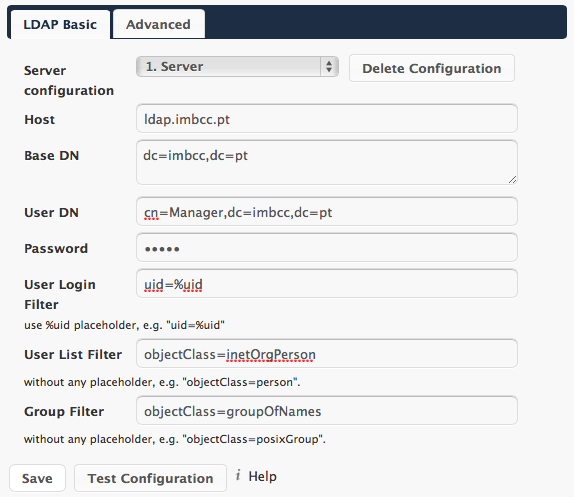
\includegraphics[width=\textwidth]{figs/oc-ldap.png}
\end{center}
\caption{Configuração básica para o LDAP no ownCloud}
\label{fig:ocbasic}
\end{figure}

O servidor ldap está em \path{ldap.imbcc.pt} e usa-se o filtro \texttt{intOrgPerson} para os utilizadores e o filtro \texttt{groupOfNames} para os grupos. A seguir preenche-se a configuração avançada como na figura~\ref{fig:ocadvanced}.

\begin{figure}[h]
\begin{center}
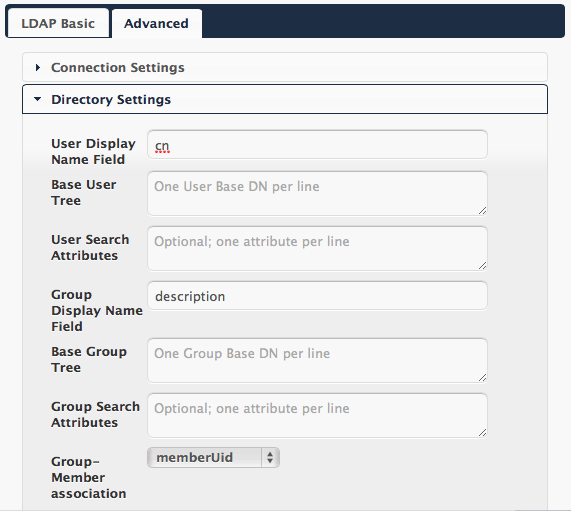
\includegraphics[width=\textwidth]{figs/oc-ldap-advanced.png}
\end{center}
\caption{Configuração avançada para o LDAP no ownCloud}
\label{fig:ocadvanced}
\end{figure}

Nas configurações avançadas usa-se o campo \texttt{cn} para mostrar o nome completo da pessoa em vez do seu username e \texttt{description} para mostrar o nome humano do grupo em vez do nome máquina.

\clearpage

\begin{figure}[h]
\begin{center}
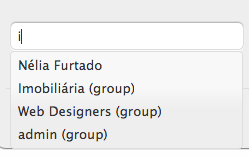
\includegraphics{figs/oc-sharing.png}
\end{center}
\caption{Resultado final quando se tenta partilhar um ficheiro.}
\label{fig:ocsharing}
\end{figure}

O resultado final deve aparecer como na figura~\ref{fig:ocsharing} ao tentar partilhar um ficheiro.

\section{FTPS}

Para se realizarem testes ao serviço de FTP seguro procedeu-se à utilização do programa lftp da seguinte forma:

\texttt{lftp -d -u vagrant,vagrant -e ``set ssl:verify-certificate no'' ftp.imbcc.pt}

\chapter{Simulação com Vagrant}

Para testar a solução encontrada, foi usado o Vagrant~\cite{Vagrant} com VirtualBox, que permite automatizar e reproduzir uma infraestrutura virtual com facilidade. Como cada máquina gasta recursos da máquina \emph{host} criou-se uma infraestrutura que pudesse simular a solução encontrada para a empresa, com o número mínimo de máquinas virtuais como se pode ver na figura~\ref{fig:virtualbox}.

\begin{figure}[H]
\begin{center}
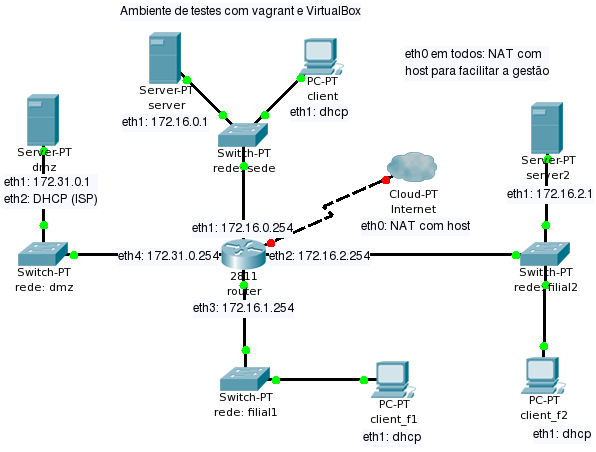
\includegraphics[width=\textwidth]{figs/diagrama-virtualbox.png}
\end{center}
\caption{Topologia de rede para simulação com o VirtualBox.}
\label{fig:virtualbox}
\end{figure}

O Vagrant\cite{Vagrant} permite automatizar através de um simples ficheiro de configuração (\texttt{Vagrantfile}) a criação de várias máquinas virtuais através do VirtualBox. O VirtualBox em si é transparente e não é preciso correr o programa nem abrir nenhuma VM através da gráfica.

Escolheu-se apenas uma imagem base para todas as máquinas para poupar espaço em disco. O endereço está no ficheiro \texttt{Vagrantfile} entregue. A primeira vez que é corrido o comando \texttt{vagrant up} na pasta do projecto é feito o download dessa imagem para o disco e daí é feita uma cópia para cada máquina virtual. A box escolhida (imagem base) foi encontrada no site Vagrantbox.es~\cite{Boxes}, tem 416MB e as seguintes características: CentOS 6.4 i386 Minimal (VirtualBox Guest Additions 4.2.12, Chef 11.4.4, Puppet 3.1.1).

\section{Particularidades}

A ligação VPN entre a Sede e a Filial~2 pode ser simulada através de uma ligação directa. Em produção teriam apenas que ser adicionadas as rotas adequadas entre os dois lados da linha. A Internet é simulada através da interface \texttt{eth0} do router que está como \emph{Host Only} (NAT). Para simular um IP dedicado para o servidor da DMZ é usada uma interface em \emph{Bridge mode} (\texttt{eth2}) com o \emph{host} que recebe o IP da nossa rede local.

O Vagrant por si só configura a primeira interface (\texttt{eth0}) em cada VM com NAT e redireccionamento para a porta 22 para que seja possível ligar individualmente por ssh a cada máquina o que facilita a gestão. Todas as outras são configuradas pelo ficheiro Vagrantfile. É portanto a interface \texttt{eth1} em modo \emph{Internal network} (\emph{intnet}) que simula as ligações locais usadas em produção. A excepção é o router que tem mais interfaces para poder interligar todas as redes.

O VirtualBox age como um switch entre interfaces \emph{intnet} com o mesmo nome. Portanto para criar o switch da sede que se pode ver na figura~\ref{fig:virtualbox}, as interfaces \texttt{eth1} do servidor e do cliente estão configuradas para a \emph{intnet} com nome \texttt{sede}, assim como a mesma interface no router para funcionar como gateway para essa rede. É o mesmo para as restantes redes.

\section{Provision com Chef}

O Vagrant apenas gere as máquinas virtuais através do VirtualBox. Para configurar as máquinas é usado um método suportado pelo Vagrant que se chama \emph{Provision}. Há várias formas de se fazer o provision, incluindo através de comandos shell. Porém preferiu-se o uso a ferramenta popular Chef~\cite{Chef}. 

Portanto quando o Vagrant activa uma máquina, depois da máquina iniciar é corrido o Chef para aplicar as configurações. Essas configurações devem ser escritas por forma a que seja possível fazer o provision tantas vezes quanto se queira para assegurar que a máquina está no estado que pretendemos.

\section{Cookbooks}

Para fazer o provision, o Chef usa \emph{cookbooks} com uma ou mais receitas (\emph{recipes}). A estrutura é simples.

Quando no Vagrantfile aparece \verb+chef.add_recipe "dns"+, o ficheiro de configuração está em \path{cookbooks/dns/recipes/default.rb}. Se a \emph{recipe} for do tipo \texttt{iptables::server} então em vez de \texttt{default.rb} é \texttt{server.rb}.

Quando uma receita usa um ficheiro (e.g. \verb+cookbook_file+), ele encontra-se em \path{files/centos/[ficheiro]} dentro do cookbook em questão. A parte do ``centos'' pode ser substituida por outra plataforma ou pelo valor ``default'' para ser usado em todos os sistemas.

Este projecto foi feito a pensar no CentOS e não são fornecidas configurações para outras plataformas.

\chapter{Guia}

É muito fácil correr este ambiente de simulação uma vez que está todo automatizado. Primeiro é preciso ter o Vagrant e o VirtualBox.

Depois de instalado o Vagrant na máquina \emph{host}, através da linha de comandos na pasta que contém o ficheiro \texttt{Vagrantfile} corre-se o comando:

\begin{verbatim}
   $ vagrant up
\end{verbatim}

Este processo, após fazer o download da box base, leva no mínimo 30 minutos para clonar essa box, iniciar as 7 máquinas, configurar as interfaces, redireccionamento de portas, etc, e aplicar as configurações (provision) que envolve fazer download dos pacotes necessários (e.g. named, http).

É também possível fazer up apenas a uma máquina:

\begin{verbatim}
   $ vagrant up dmz
\end{verbatim}

Ou a todas as máquinas clientes usando uma expressão regular:

\begin{verbatim}
   $ vagrant up /client*/
\end{verbatim}

\emph{Nota: Os nomes das máquinas usadas pelo vagrant estão representados na figura~\ref{fig:virtualbox}.}

Depois do primeiro \texttt{up} pode-se saltar o provision para ser mais rápido:

\label{noprovision}
\begin{verbatim}
   $ vagrant up server --no-provision
\end{verbatim}

Só faz sentido usar o comando \texttt{up} quando uma máquina não está a correr. Para reiniciar usa-se o \texttt{reload} ou para encerrar usa-se o \texttt{halt}.

Também existe o \texttt{suspend} e o \texttt{resume} para colocar em estado de suspensão. Assim poupa-se RAM mas não espaço em disco.

No final pode-se destruir tudo com (máquinas criadas e box base):

\begin{verbatim}
   $ vagrant destroy -f
   $ vagrant box remove centos virtualbox
\end{verbatim}

\section{Usar o servidor DNS externamente}

Durante o provision o IP público/externo atribuído à DMZ é actualizado automaticamente no servidor DNS para que seja possível acedê-lo fora do ambiente privado do VirtualBox.

É fornecido um script que verifica e actualiza o IP no DNS caso este tenha mudado. Em todo o caso o IP actual é impresso no ecrã e pode ser usado para actualizar na lista de nameservers da máquina host para que se possa utilizar a resolução de nomes da nossa rede virtualizada.

Portanto para saber o IP da dmz:

\begin{verbatim}
   $ ./dns.sh
   Already up to date for IP 192.168.1.131!
\end{verbatim}

No entanto se a máquina já tiver sido iniciada e esse IP mudou por algum motivo (e.g. deslocamento para outra rede), também dá para reiniciar a interface para que seja renovado o IP atribuido e actualizar o servidor DNS:

\begin{verbatim}
   $ ./dns.sh -r
   Determining IP information for eth2... done.
   Recovering from backup... done.
   Updating files... done.
   Stopping named: .[  OK  ]
   Starting named: [  OK  ]
   Your nameserver is at 192.168.0.105
\end{verbatim}

O script que faz esse update pode ser consultado em \path{cookbooks/dns/files/centos/dns-external.sh}.

Durante o update os ficheiros originais são guardados num backup (ficheiro terminado em \textasciitilde). Esse ficheiro original depois é recuperado para fazer novo update simplesmente substituindo as referências ao IP interno pelo novo IP externo.

\section{Acesso SSH às máquinas}

Cada máquina pode ser acedida individualmente através do comando \texttt{vagrant ssh [vm]}. Esse acesso é criado automaticamente pelo Vagrant através da interface \texttt{eth0} em NAT com port forwarding que é gerido automaticamente.

Esse acesso facilita a gestão das máquinas mas para simular o que aconteceria em produção acede-se à dmz externamente e daí novo ssh para qualquer máquina interna. Uma vez que o Vagrant também cria em cada máquina automaticamente o utilizador \texttt{vagrant} com poderes administrativos, aproveitou-se esse utilizador na configuração dos servidores \texttt{sshd} para ser o único com acesso.

Para acesso root ao servidor interno:

\begin{verbatim}
   $ ssh vagrant@imbcc.pt
   vagrant@imbcc.pt's password: 
   [vagrant@dmz ~]$ ssh vagrant@server
   vagrant@server's password: 
   [vagrant@server ~]# su -
   Password:
   [root@server ~]# 
\end{verbatim}

A password do utilizador \texttt{vagrant} e \texttt{root} é \texttt{vagrant}.

\section{Pasta partilhada}

O Vagrant configura em cada VM automaticamente uma pasta \path{/vagrant} que aponta para a pasta no host onde está o ficheiro \path{Vagrantfile}. Isso pode ser útil para transferir ficheiros de um lado para o outro e é o que usamos para exportar as configurações das máquinas.

\section{Ordem de iniciação}

A ordem pela qual se iniciam as máquinas tem importância uma vez que há dependências entre elas. A máquina \texttt{dmz} tem ligação própria à Internet e portanto pode ser usada independentemente, excepto pelo ownCloud que precisa do LDAP do \texttt{server}.

Todas as outras máquinas precisam do \texttt{router} para poderem aceder à Internet e da \texttt{dmz} para a resolução de nomes, incluindo o próprio \texttt{router}.

\section{Problemas}

Se uma máquina não conseguir aceder à Internet irá falhar na fase do \emph{provision}. Se a máquina já tiver sido construída pode-se saltar essa fase com a opção \verb+--no-provision+ como visto no início do capítulo \ref{noprovision}~\nameref{noprovision}.

Também por vezes pode acontecer uma máquina não responder quando se encerra ou inicia. Pode aparecer um erro do tipo:

\begin{verbatim}
   stderr: VBoxManage: error: The object is not ready
\end{verbatim}

Nesses casos é preciso insistir.

Para erros durante a fase do provision pode-se fazer novo provision sem reiniciar a máquina:

\begin{verbatim}
   $ vagrant provision server
\end{verbatim}

\chapter{O que falta}

Faltou fazer ligação segura por TLS entre o ownCloud e o servidor LDAP. Também faltou usar o LDAP com o FTPS para autorizar o grupo da imobiliária nos seus \emph{userdirs} e os web designers à pasta \path{/var/www} e certificar que ele funciona bem no geral.

\begin{thebibliography}{9}
\addcontentsline{toc}{chapter}{Referências}
\phantomsection

\bibitem{Vagrant} Vagrant, \emph{Development environments made easy.}, disponível em\\
\small{\url{http://www.vagrantup.com}}

\bibitem{Boxes} Vagrantbox.es, \emph{A list of boxes for Vagrant}, disponível em\\
\small{\url{http://www.vagrantbox.es}}

\bibitem{Chef} Chef, \emph{infrastructure as code}, disponível em\\
\small{\url{http://www.opscode.com/chef/}}

\end{thebibliography}

\end{document}